\documentclass{article}
\usepackage[utf8]{inputenc}
\usepackage{graphicx}
\graphicspath{ {./images/} }
\title{Real analysis and hol light}
\author{Palash }
\date{January 2020}

\begin{document}

\maketitle

\section{Question}
\textbf{How to create real number from scratch?
} \newline
\textbf{What is an ordered field ?}\newline
In order to describe ordered filed first we understand what is field and what is ordered relation\\
{
What is a field?
}\\
It is set f with two binary operations: Addition , Multiplication 
Any set which satisfy associative, commutative, distribute,commutative, inverse then such called call set of field OR we can say these are the property of field set. \\
Example: Set of rational number, Set of Real numbers\\
Answer: \\
A field(f + .) is an ordered field if the following properties are satisfied \\
\vspace{2mm}
\\
Trichotomy property\\
Transitive property\\
Addition composition\\
Multiplication composition\\
\\
Some other points:\\

\textbf{Supremum}: In simple words least upper bound is called supremum \\

\textbf{Infimum}:  Greatest lower  bound  \\
\\
\textbf{complete ordered field:
}\\
When an ordered field is bounded above and bounded below. In other \textbf{words When supremum and infimum  values are coming in ordered field then we will say that field is complete ordered field}
\\
\\
\\
Construction of real number\\
\\
Synthetic approach (Reference from Wikipedia)\\
\\
Synthetic approach defined real number system as a complete ordered field 
Such that real number system consist of set R two distinct elements 0 and 1 of R, two binary operations + and × on R.\\
\\
\\
\\
\\
\textbf{Cauchy Sequence }\\
\\
Whats is Cauchy sequence ?\\
A sequence is said to be a cauchy sequence  for every epsilon greater than zero.There is a positive integer m          m, n > N then |am- an| < ε. For all m>n \\
\\
First we will construct Natural Numbers:
\\
Constructing Real numbers with Peano’s Axiom
\\
\vspace{5mm} %5mm vertical space

\textbf{Axioms:}
\\*
\begin{enumerate}
\item There exist a natural number 1
\item If a is a natural number, then its successor  s(a) = a+1 is also a natural number.
\item 1 is not the successor is any natural number
\item If two numbers have the same successor then they must be the same number.
\item Given a set S, if 1 belongs to S and contains the successor of any number in S then S must contain all of the natural numbers.\\
\end{enumerate}
\\
\textbf{6/01/2020}
\\
\\
\textbf{Some basic definition:
}\\
\\
\textbf{Least element}:  Let A is subset of Q where Q is a set of all Rational number, r  Q then r is said to be least element of A only if
r {\in} A:r {\leq x} ,{\forall} x {\in} A. \\   
\\
\\
\textbf{Largest element:}  Let A is subset of Q where Q is a set of all Rational number, u {\in} Q then u is said to be Largest element of A only if
u {\in} A
u {\geq} x, for all x belongs A
\\
\\*
(This definition is in my own words may be not like standard definition)\\
\\
\textbf{Dedekind Cuts:}  Since the set of rational is an ordered field so  we can arrange this set of rational number Q on number line. Suppose we mark a cut P on that number line such that it divides number line in two parts or in two sub set of Q.
\\
\\
\textbf{08/01/2020
}\\
\\
Studying Hol light Code\\
\\
\\
\textbf{File name: Lib.ml}
\\
Functions Explantion\\
https://www.cl.cam.ac.uk/~jrh13/hol-light/HTML/map.html\\
\\
Starting file for hol light\\
https://github.com/jrh13/hol-light/blob/master/lib.ml\\
\textbf{map}\\
\\
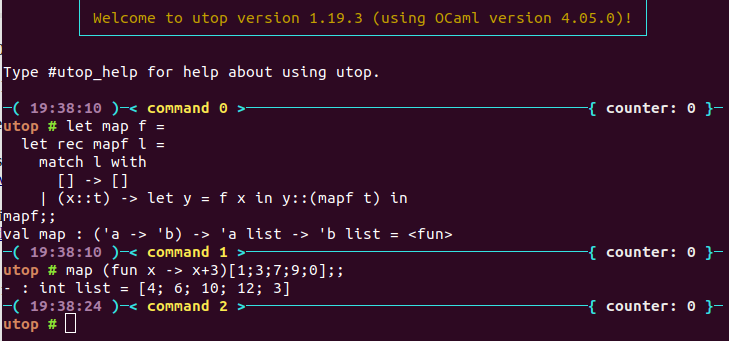
\includegraphics{images/image4.png}
\\
Takes funtion and list and appiles function to each element of list:\\
\\
\\
\textbf{last}\\
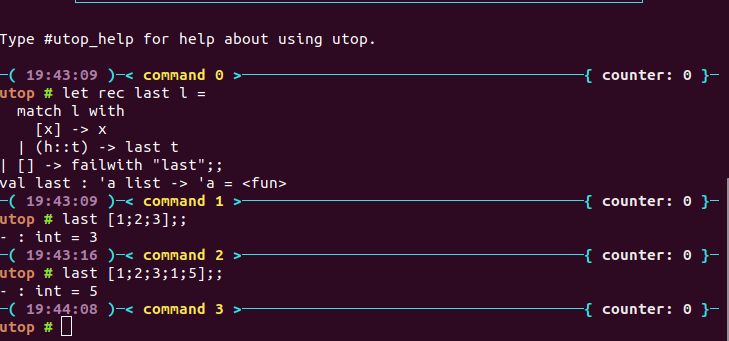
\includegraphics{images/image10.png}
\\
\\
This functions takes List and return last element of the list
and if list is empty then exception: Failure "last".\\
\\
\textbf{butlast}\\
\\
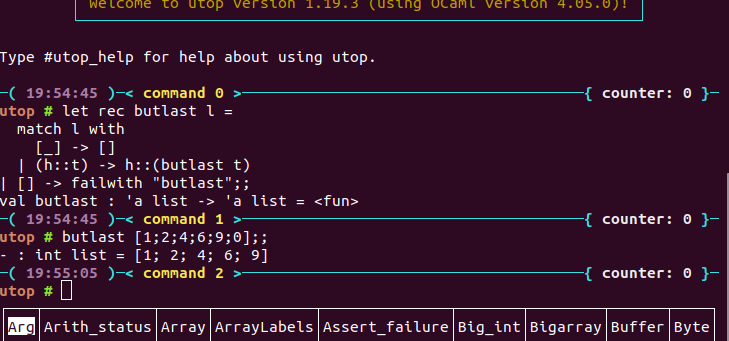
\includegraphics{images/image9.png}
\\
as you can see in screenshot this function gives list except last element.\\
butlast [1;2;4;6;9;0];; \\
- : int list = [1; 2; 4; 6; 9] \\
\\
\\
\textbf{el}\\
\\
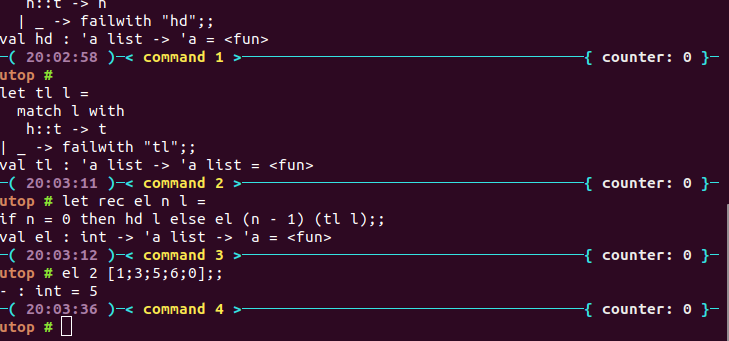
\includegraphics{images/image8.png}
\\
el function gives specfied element from list
Consist of two other function hd , tl  specifies in lib.ml \\
\\
\\
\textbf{rev}\\
\\
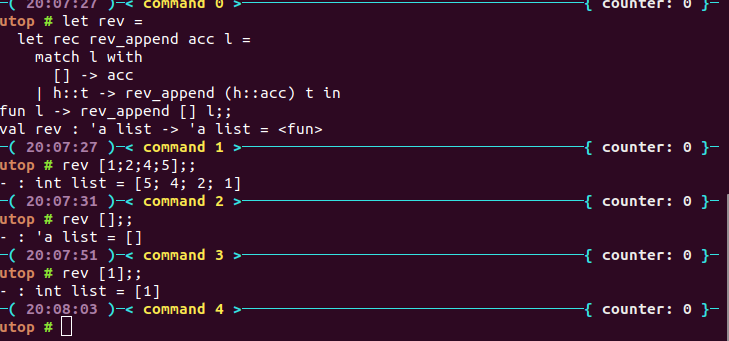
\includegraphics{images/image5.png}
\\
\\
return reversed list\\
\\
\textbf{map2}
\\
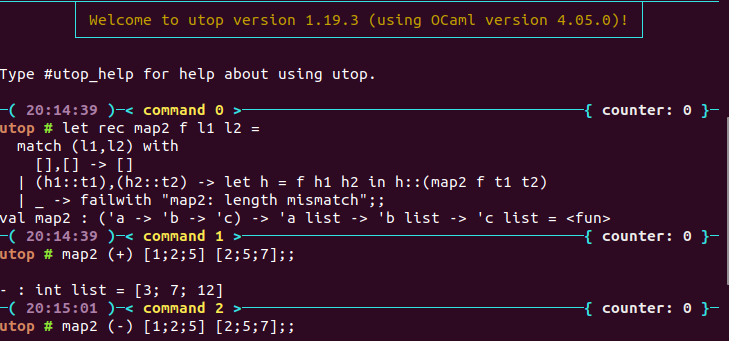
\includegraphics{images/image3.png}
\\
maps2 take two list and function and gives new list\\
map2 f ([x1;...;xn],[y1;...;yn]) returns [f(x1,y1);...;f(xn,yn)].\\
\\
\textbf{funpow}
\\
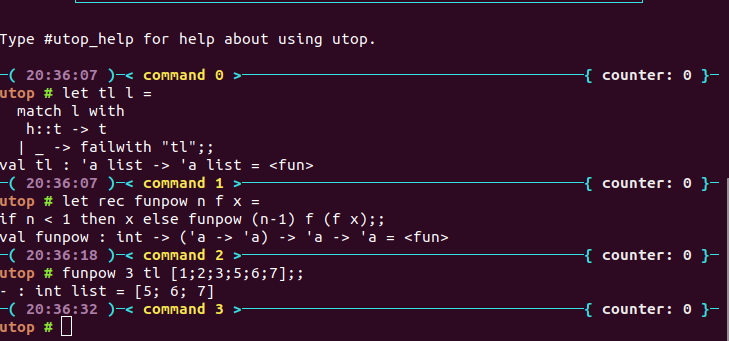
\includegraphics{images/image11.png}
\\
This function takes 3 argument: int -> ('a -> 'a) -> 'a -> 'a = <fun>\\
how many times n a function f applies to x
\\
\\
\textbf{itlist}
\\
\\
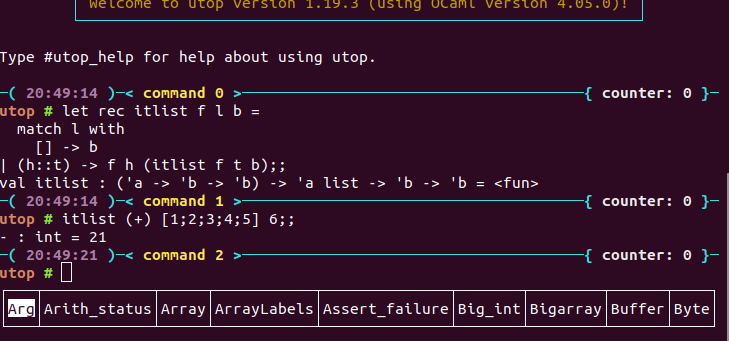
\includegraphics{images/image2.png}
\\
\\
This function applies function f to adjacent element of list\\
\\
\\
\textbf{SET OPERATIONS ON LIST:
}\\
\\
\textbf{mem}\\
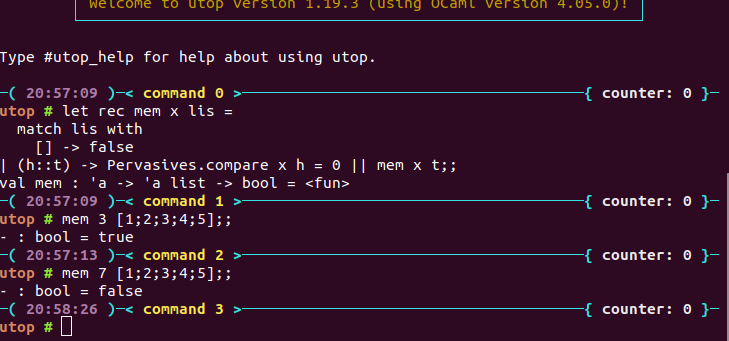
\includegraphics{images/image7.png}
\\
mem is a boolen type function\\
returns true if given element is present in list else return false\\
\\
\\
\textbf{Insert}\\
\\
\\
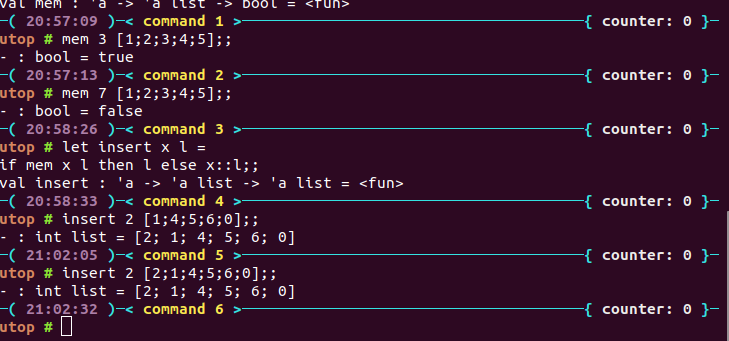
\includegraphics{images/image12.png}
\\
\\
insert function checks element is present in list if not the insert that element in that list\\
\\
\\
\textbf{union}\\
\\
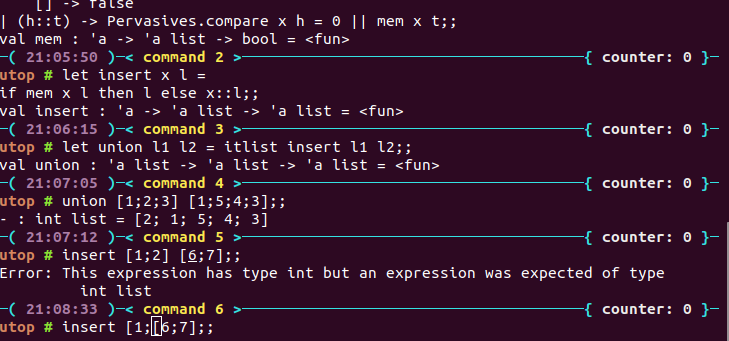
\includegraphics{images/image6.png}
\\
\\
Union returns a list consisting of the elements of l1 not already in l2 concatenated with l2\\
\end{document}
